\chapter{Tecnolog\'ia ARM}\label{ch:tecnologia_arm}

Para alcanzar nuestros objetivos necesitamos encontrar un punto de
arranque y para ello buscamos entre la tecnología que se ofrece actualmente
a la comunidad.

Para poder crear sistemas con capacidades específicas como video,
audio ó WiFi podemos utilizar varias estrategias, desde diseñar un
sistema utilizando transistores hasta programar una arquitectura existente
en lenguajes como .NET o Java.

Cada una de estas opciones tiene sus ventajas y desventajas. Si trabajamos
con tecnologías de alto nivel tenemos un tiempo de desarrollo rápido
y no se necesitan muchos conocimientos sobre la arquitectura, con
el costo de que no podemos hacer modificaciones a la arquitectura,
es decir dependemos del fabricante para incluir nuevas funcionalidades
en el sistema. Si en cambio trabajamos con tecnologías de bajo nivel
se necesita un mayor grado de conocimientos, y los tiempos de desarrollo
se elevan.

En nuestro caso, tenemos interés en ser capaces de modificar la plataforma
de hardware para agregar nueva funcionalidad o incluso tener la capacidad
de hacer modificaciones a la arquitectura, teniendo al mismo tiempo
cierta facilidad para el desarrollo de aplicaciones.

Por esto, necesitamos una base mínima, y decidimos que para ello podíamos
utilizar un microcontrolador, pues nos da la capacidad de hacer cómputo
de distintos tipos de una manera más adecuada. 


\section{Elecci\'on de la tecnolog\'ia}

Una vez tomada esta decisión, se debe de elegir una tecnología que
cumpla con nuestros requerimientos, los cuales deben de ser:
\begin{itemize}
\item Accesible.
\item Fácil acceso a la documentación.
\item Flexible, que la arquitectura permita hacer aplicaciones variadas.
\item Confiable.
\end{itemize}
Teniendo estos parámetros en cuenta se definieron una serie de tecnologías
que pudieran cumplir nuestros requerimientos, las tecnologías seleccionadas
para la revisión fueron las siguientes:
\begin{itemize}
\item \ac{ARM}
\item Blackfin
\item \ac{MIPS}
\item \ac{PIC}
\end{itemize}
Cada una de estas opciones tiene sus ventajas y desventajas, \ac{ARM}
y \ac{MIPS} son estándares que permiten que los fabricantes que lo
deseen implementen sus circuitos integrados y haya cierto grado de
interoperabilidad entre ellos. Blackfin es interesante, pues se trata
de un esfuerzo de \emph{{}``Open Hardware'' }con lo que es posible
implementar mejores desde el nivel más bajo. La tecnología \ac{PIC},
de Microchip es una de las más difundidas y más sencillas de usar,
sin embargo no se ha contemplado para controlar un dispositivo de
propósito general, como un dispositivo móvil o incluso un dispositivo
para videojuegos.%
\begin{table}
\begin{tabular}{|c|c|c|c|c|c|}
\cline{2-6} 
\multicolumn{1}{c|}{} & ARM & Blackfin & MIPS & PIC & ARM.\tabularnewline
\hline 
MMU & Sí & Sí & Sí & No & RISC\tabularnewline
\hline 
Libre & No & Sí & No & No & RISC\tabularnewline
\hline 
Flexible & Sí & No & Sí & Sí & RISC\tabularnewline
\hline 
Accesible & Sí & No & Sí & Sí & RISC\tabularnewline
\hline
\end{tabular}

\caption{\label{tab:comp-tec-table}Comparación de tecnologías}

\end{table}


Como podemos ver en la tabla \ref{tab:comp-tec-table}, las tecnologías
ARM y MIPS son las que más se acercan a nuestros requerimientos, aunque
no cuentan con la ventaja de ser libres, sin embargo tienen algunas
características importantes. Al ser estándares, los fabricantes pueden
crear sus microcontroladores con diferentes capacidades para usos
muy variados. 

Otra ventaja de ambas tecnologías es que soportan dispositivos con
y sin MMU, con lo que se pueden utilizar sistemas operativos como Linux
y Windows CE en caso de ser necesario.

En los últimos años la tecnología \ac{ARM}, como se puede ver en
las siguientes imágenes, ha dominado gran parte del mercado de los
dispositivos y los pronósticos indican que seguirá creciendo. Casi
todos los fabricantes lo utilizan para sus dispositivos móviles incluso
con ejemplos como el iPhone o el Google Android.

%
\begin{figure}
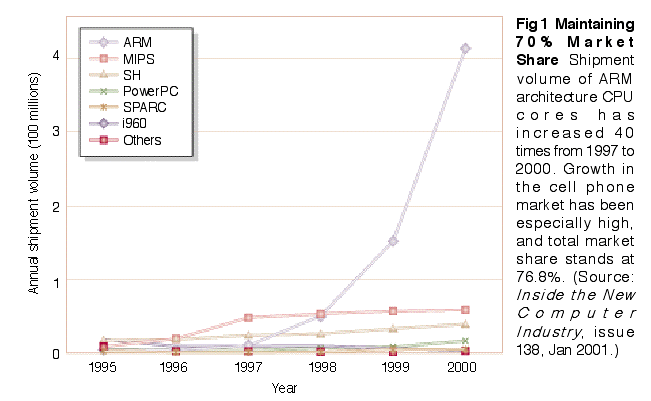
\includegraphics[scale=0.5]{img/tablaarm1}

\caption{Uso de tecnología ARM hasta el 2000{\scriptsize }\protect \\
{\scriptsize http://www.designreuse.com/news img/20090430 microprocessormarketforecast.gif}}



\end{figure}


{\scriptsize{} }%
\begin{figure}
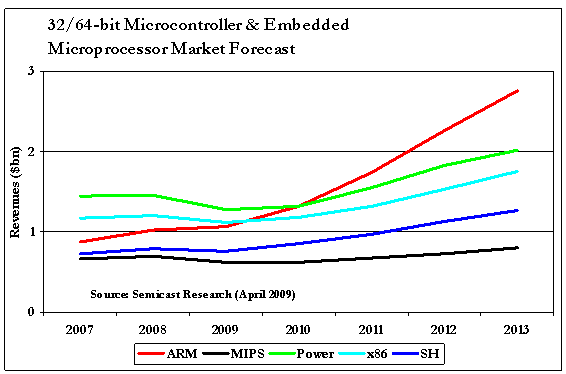
\includegraphics[scale=0.5]{img/tablaarm2}

{\scriptsize \caption{Predicción del uso de tecnología ARM hasta el 2013\protect \\
{\scriptsize http://www.designreuse.com/news img/20090430 microprocessormarketforecast.gif }}
}{\scriptsize \par}


\end{figure}


